\documentclass[letterpaper,12pt]{article}
\usepackage[spanish]{babel}
\spanishdecimal{.}
\usepackage[utf8]{inputenc}
\usepackage{graphicx}
\usepackage{caption}
\usepackage{subcaption}
\usepackage[top=2.5cm, bottom=2.5cm, left=2.5cm, right=2.5cm]{geometry}
\usepackage{hyperref}
\usepackage{verbatim}

\title{Práctica 4  \\ Creación de una mapa de celdas de ocupación mediante el paquete \texttt{gmapping}}
\author{M.I. Marco Negrete}
\date{Robots Móviles y Agentes Inteligentes}
\begin{document}
\renewcommand{\tablename}{Tabla}
\maketitle
\section*{Objetivos}
\begin{itemize}
\item Crear un mapa del Laboratorio de Biorrobótica que sea útil para las tareas de navegación que se implementarán en las siguientes prácticas. 
\item Familiarizar al alumno con el uso del paquete GMapping para creación de mapas geométricos.
\item Familiarizar al alumno con la adquisición de lecturas del sensor láser Hokuyo UG01.
\end{itemize}

\section{Introducción}
Las celdas de ocupación son un tipo de mapa geométrico en el que el espacio se discretiza con una determinada resolución. Cada una de las celdas (o pixeles en el caso de espacios bidimensionales) tiene un valor asignado que indica el nivel de ocupación del espacio que ésta representa. En general el nivel de ocupación es booleano, esto es, cada celda puede tener sólo dos valores: espacio libre o espacio ocupado. En caso de usar un enfoque probabilístico, el valor de cada celda indica la probabilidad de que esté ocupada. 

ROS tiene el mensaje \texttt{OccupancyGrid}, dentro del paquete \texttt{nav\_msgs}, para representar este tipo de mapas. En este mensaje, el valor de ocupación de cada celda se representa con un entero en el intervalo $[0,100]$. El valor de -1 indica que no se tiene información sobre la celda. 

El paquete \texttt{gmapping} sirve para crear celdas de ocupación a partir de las lecturas de un sensor láser y de la odometría calculada por la base móvil. El mapa generado se puede guardar en una imagen utilizando el paquete \texttt{map\_server}.

\section{Desarrollo}
\textbf{Nota:} Para esta práctica se asume que el alumno ejecutó correctamente las prácticas 1 y 2.

\subsection{Prerrequisitos}
Como primer paso, asegúrese de actualizar y recompilar el repositorio mediante los comandos:
\begin{verbatim}
cd ~/RoboticsCourses
git pull origin master
cd catkin_ws
catkin_make
\end{verbatim}

Antes de poder utilizar el hardware, es necesario configurar los nombres que el sistema operativo asignará al sensor láser, joystick y base móvil, para ello ejecute los siguientes comandos:
\begin{verbatim}
sudo cp ~/RoboticsCourses/Prerequisites/80-justinaRobot.rules /etc/udev/rules.d/
sudo udevadm control --reload-rules
sudo service udev restart && sudo udevadm trigger
\end{verbatim}

Además, es necesario instalar el paquete \texttt{gmapping} con el comando:
\begin{verbatim}
sudo apt-get install ros-indigo-gmapping
\end{verbatim}

\subsection{Creación del mapa}
En el laboratorio se dispone de dos bases móviles para realizar las pruebas: JustinaCN y JustinaNL. Las figuras \ref{fig:JustinaCN} y 
\ref{fig:JustinaNL} son fotos de las dos bases disponibles. 

\begin{figure}
\centering
\begin{subfigure}{0.45\textwidth}
  \centering
  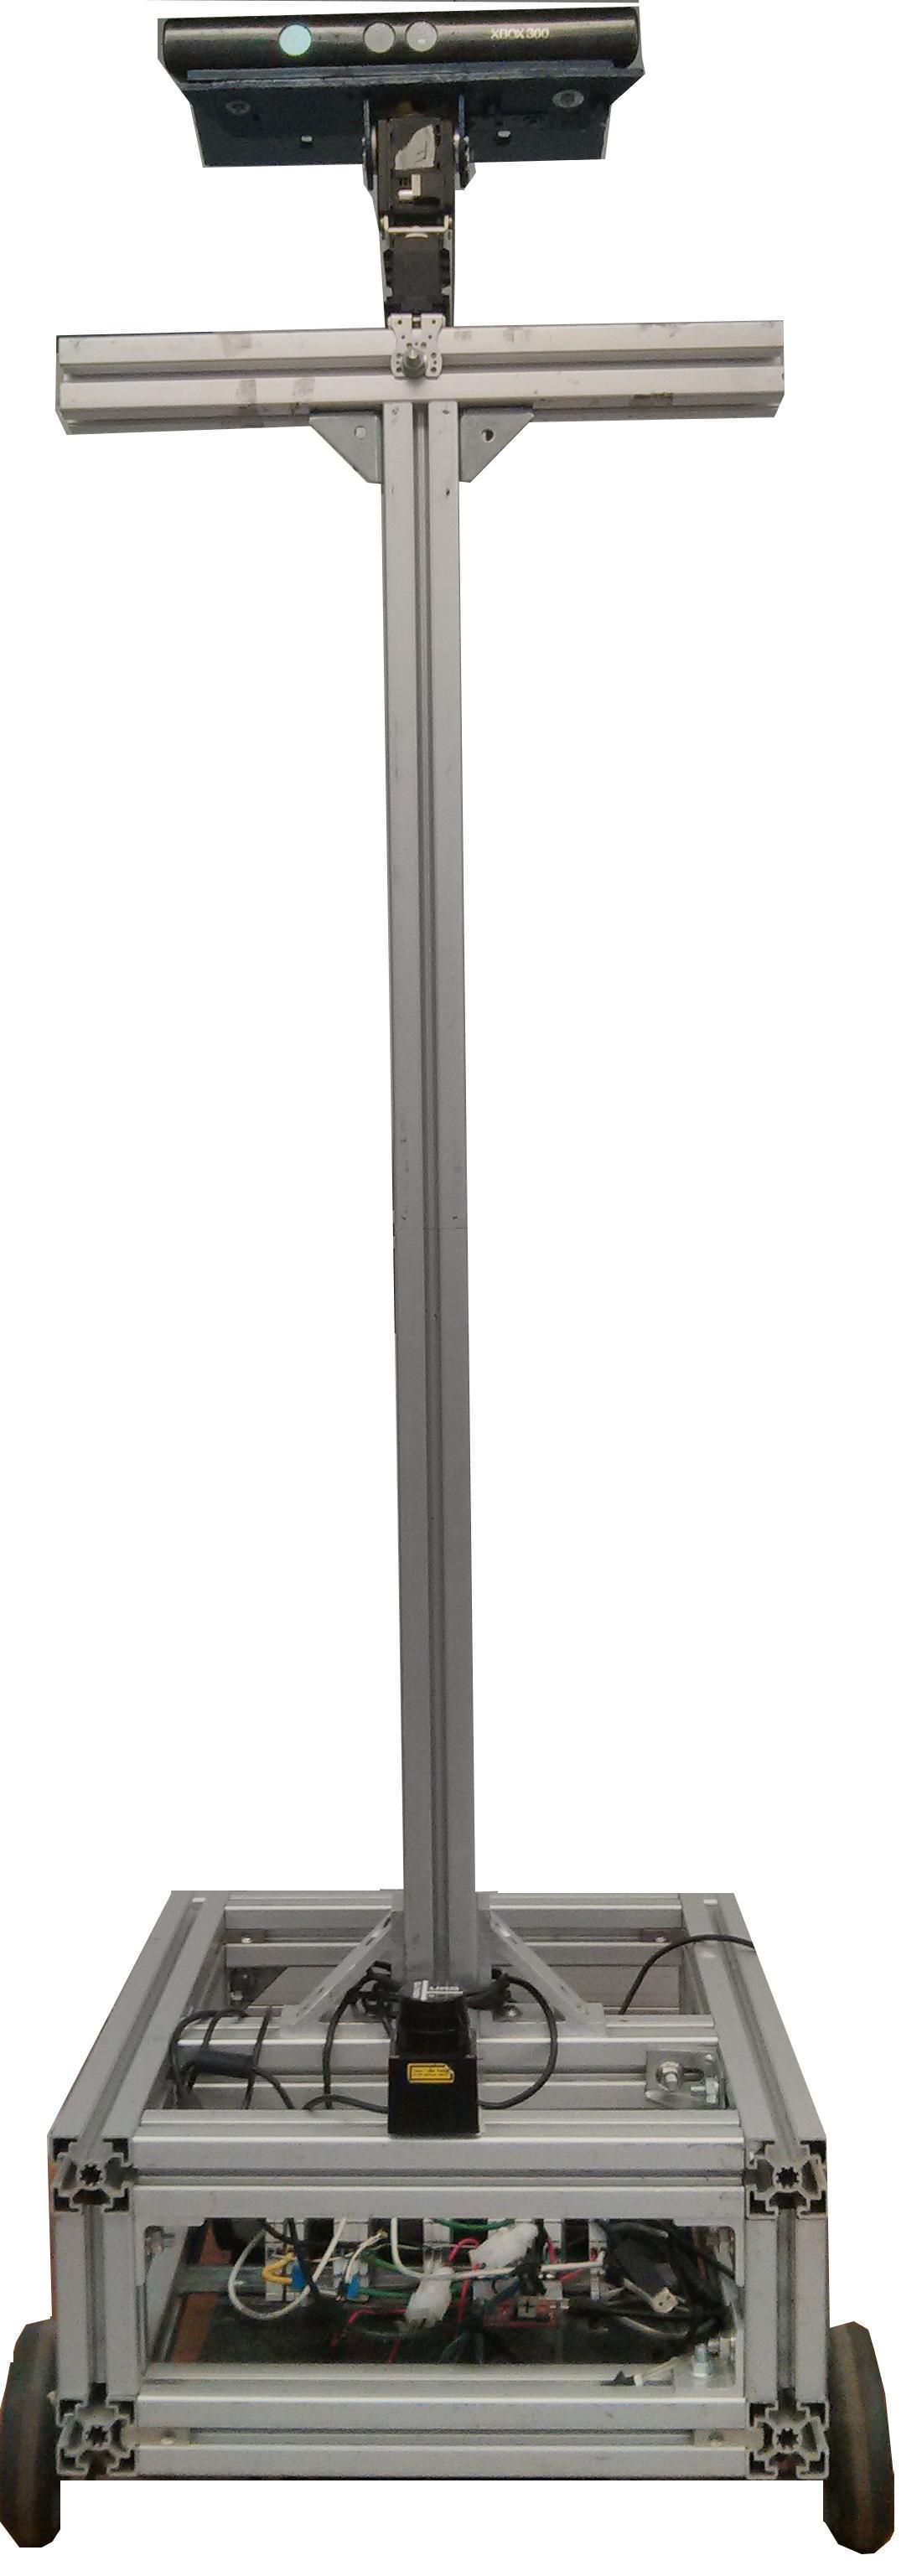
\includegraphics[width=0.5\textwidth]{Figures/JustinaCN.jpg}
  \caption{JustinaCN}
  \label{fig:JustinaCN}
\end{subfigure}
\begin{subfigure}{0.45\textwidth}
  \centering
  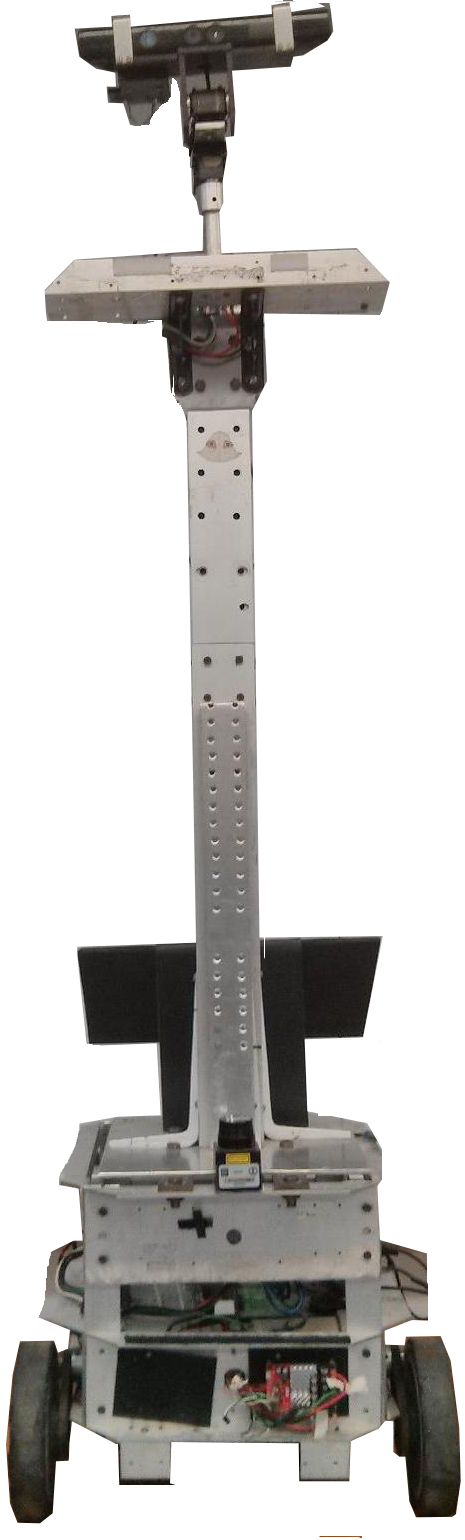
\includegraphics[width=0.5\textwidth]{Figures/JustinaNL.jpg}
  \caption{JustinaNL}
  \label{fig:JustinaNL}
\end{subfigure}
\caption{Bases móbiles disponibles en el Laboratorio de Biorrobótica}
\end{figure}

Para comenzar a crear el mapa con JustinaCN, conecte el cable USB etiquetado como ``USB_Main'' a cualquier puerto de la computadora y ejecute el comando:
\begin{verbatim}
roslaunch bring_up mapping_justinaCN
\end{verbatim}

Si se utiliza a JustinaNL, ejecute el comando:
\begin{verbatim}
roslaunch bring_up mapping_justinaNL
\end{verbatim}

En ambos casos se ejecutarán varios nodos, de los cuales, los más importantes son: \texttt{gmapping}, \texttt{hokuyo\_node} y \texttt{mobile\_base}. El visualizador debe mostrar algo parecido a la figura \ref{fig:rviz}.

\begin{figure}
\centering
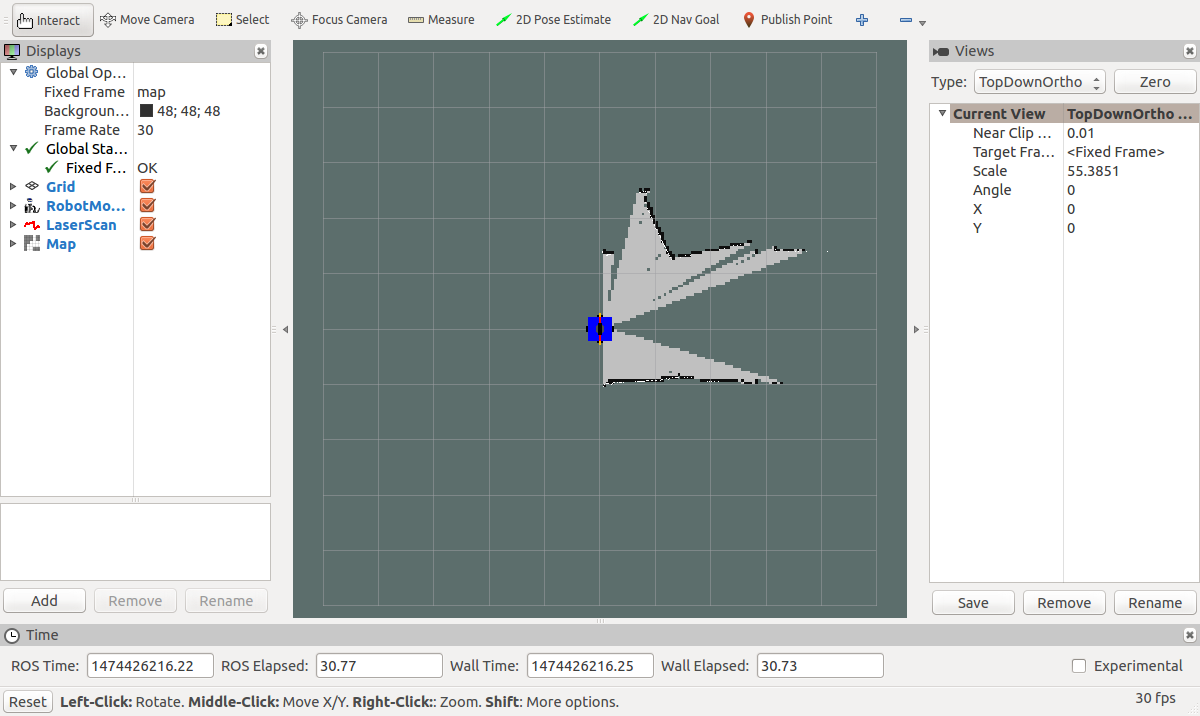
\includegraphics[width=0.9\textwidth]{Figures/rviz_mapping.png}
\caption{Ejemplo de lo que  muestra el visualizador al comienzo del mapeo}
\label{fig:rviz}
\end{figure}

Las bases móbiles se teleoperan con el \textit{stick} derecho del joystick. Para crear el mapa, basta con mover la base por todo el espacio que se quiera representar. El mapa se actualiza cada que el robot se mueve una distancia de 30 [cm] o gira un ángulo de 0.2 [rad]. Es importante no mover la base muy rápido para que el mapa se pueda crear correctamente. 

Si el mapa dibujado en el visualizador comienza a mostrar espacios incongruentes será necesario comenzar el mapeo nuevamente. Basta con detener el proceso y ejecutar nuevamente el comando \texttt{roslaunch}. Es probable que se requieran varios intentos para obtener un buen mapa. 

Una vez que se ha mapeado todo el espacio deseado, ejecute, \textbf{desde otra terminal, sin detener los procesos previos}, el siguiente comando:
\begin{verbatim}
rosrun map_server map_saver -f ~/RoboticsCourses/catkin_ws/src/student/biorobotics_map
\end{verbatim}
Este comando guarda el mapa en la carpeta \texttt{student} (creada en clase); dicho mapa se guarda en dos archivos, uno con extensión \texttt{.pgm} (el mapa en sí), que puede ser abierto por un visualizador de imágenes, y un archivo \texttt{.yaml}, que contiene información relativa al mapa. 

Compare la imagen con el ambiente real. Si la representación no es suficientemente buena, repita el proceso completo. La figura \ref{fig:mapa} es un ejemplo de un mapa obtenido con este proceso. 

\begin{figure}
\centering
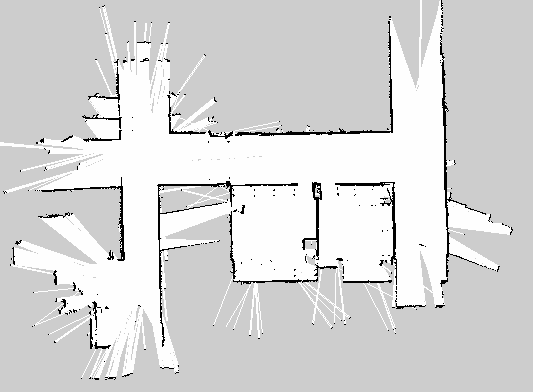
\includegraphics[width=0.7\textwidth]{Figures/map.png}
\caption{Ejemplo de un mapa}
\label{fig:mapa}
\end{figure}


\section{Evaluación}
\begin{itemize}
\item La práctica se considera entregada si el mapa representa al ambiente de manera satisfactoria. 
\end{itemize}

\end{document}